\subsection{Layer Qualities with Computational \RTransforms}
\label{sxn:empirical_comp_r_transforms}

In this Section, we look at how the \HTSR layer quality HT PL metric $\alpha$
compares to computing the \LayerQualitySquared $\QT$ using
the Computational \RTransform method proposed in Section~\ref{sxn:comp_rmt}
for fully trained MLP3 model(s).
Figure~\ref{fig:MLP3_qualities}
presents results for FC1 and FC2 layers, comparing
both the batch size and the mean $\alpha$ metric to the
mean $\QT$, and the results are quite different.


\begin{figure}[h]
    \centering
    \subfigure[FC1 batch size vs $\QT$]{
        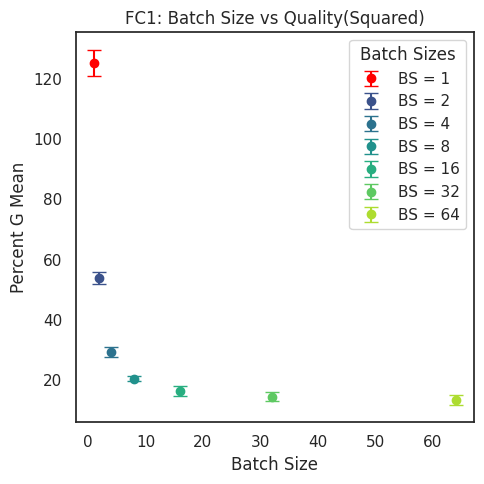
\includegraphics[width=6cm]{img/FC1_bs_vs_Q.png}
        \label{fig:FC1_bs_vs_Q}
    }
    \hspace{1cm} % Add space between subfigures
    \subfigure[FC1 Layer $\alpha$ vs $\QT$]{
        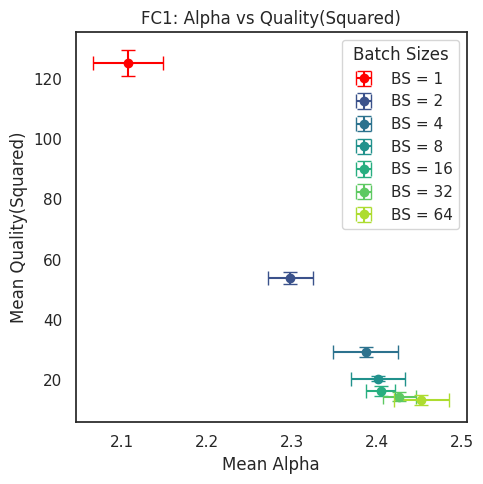
\includegraphics[width=6cm]{img/FC1_alpha_vs_Q.png}
        \label{fig:FC1_alpha_vs_Q}
    }
    \hspace{1cm} % Add space between subfigures
    \subfigure[FC2 batch size vs $\QT$]{
        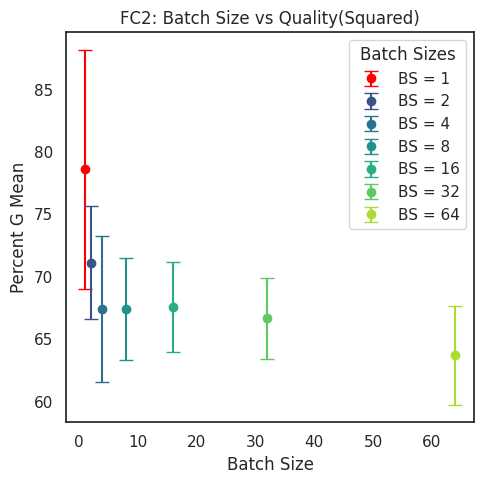
\includegraphics[width=6cm]{img/FC2_bs_vs_Q.png}
        \label{fig:FC2_bs_vs_Q}
    }
    \hspace{1cm} % Add space between subfigures
    \subfigure[FC2 Layer $\alpha$ vs $\QT$]{
        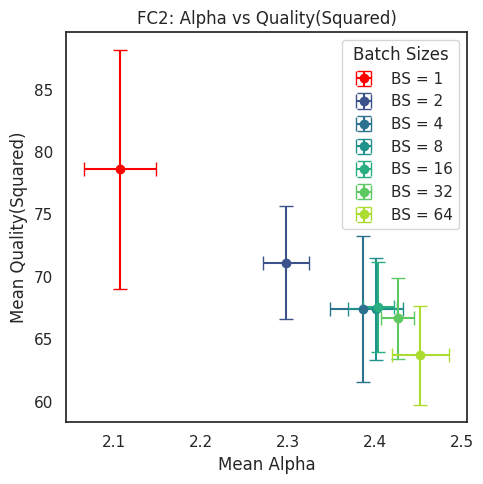
\includegraphics[width=6cm]{img/FC2_alpha_vs_Q.png}
        \label{fig:FC2_alpha_vs_Q}
    }
    \caption{
      Evaluation of the computational \RTransform \LayerQualitySquared metric $\QT$
      on the fully trained MLP3 model(s) for different batch sizes.
    }
    \label{fig:MLP3_qualities}
\end{figure}


For FC1, as shown in Figure~\ref{fig:FC1_bs_vs_Q}, the quality metric \(\QT\) increases as the batch size decreases, following the expected trend. Notably, for batch size = 1, the quality metric exceeds $100\%$,
which suggests that the layer may be overfit in this scenario, which is similar to results obtained earlier. Furthermore, in Figure~\ref{fig:FC1_alpha_vs_Q}, the quality metric \(\QT\) shows a strong correlation with the $\alpha$ metric, consistent with the theoretical predictions of the \HTSR framework.
Earlier results suggest that the FC1 layer captures most of the correlation in the data,
so it is interesting that this layer also has much smaller error bars, indicating more consistent quality across different batch sizes.

In contrast, for FC2, while the general trends are similar (as shown in Figures~\ref{fig:FC2_bs_vs_Q} and~\ref{fig:FC2_alpha_vs_Q}), the error bars on the quality metric $\QT$ are much larger. This indicates significantly higher variability in computational quality compared to FC1. The large error bars for FC2 suggest that, while the $\QT$ metric is theoretically grounded, it is less effective than the existing \HTSR layer quality metric $\alpha$, which exhibits greater stability and reliability in capturing layer behavior. These differences highlight the distinct computational characteristics of the two layers, with FC1 demonstrating more predictable trends that align closely with theoretical expectations.

